\subsection{Development approach} 
To begin identifying an appropriate development methodology, it was necessary to firstly understand 
the project requirements. The project requirements and features were agreed over a number of 
meetings with the primary stakeholders.

The two most preferred development methodologies were 
Scrum and XP(Extreme Programming). Scrum is an agile project management technique that focuses more 
on the management of software development projects. The product is completed in a series of one to 
four week iterations, or sprints as they are called. Before each sprint, a planning meeting is held 
to determine which features will be implemented during that sprint. Similarly, XP is an agile 
methodology which is designed for small, co-located teams aiming to get quality and productivity as 
high as possible. It does this through the use of rich, short, informal communication paths with 
emphasis on skill, discipline and understanding at the personal level, minimizing all intermediate 
work products.

It was decided amongst the group that combining characteristics form both methods 
would be the most beneficial way, merely because Scrum focuses on the project management whereas XP 
on the programming part.

Managing efficiently the development lifecycle of the project was a very 
important task for the team to work properly. Meetings with the supervisor took place each week 
where the project progress was thoroughly discussed as well as more feasible features to be 
implemented. In addition, various issues were brought up in order to provide solutions. Except from 
the meetings with the supervisor, the team had its own weekly meeting for keeping up with what 
everyone has been doing for the last week. New tasks were also assigned to members of the team. For 
every meeting an agenda was stored in an online document containing information about the team 
members absent, location, action items and topics to be discussed. In the end of the meetings tasks 
were assigned, managed or archived using an online visual board, similar to Scrum Board, to 
encourage a more agile development.

As regards to the XP approach, it was proved that adopting 
some of its techniques would significantly improve the development process. More specifically, pair 
programming was effectively put in use. Team members where working in pairs whenever possible to 
develop a single feature. Additionally, XP promotes test-driven development. As mentioned in the 
first report, testing would be rather difficult due to the nature of the project being partly 
research based. However, essential tests were implemented in the server to validate the classifier 
as well as blackbox tests for the correctness and responsiveness of the rest API server. 

Throughout the development, various technologies had to be used and implemented. According to each 
members skills these elements were divided in such ways to effectively use the members previous 
experience. The team was also split to different design aspects of the project; however, more on the 
team structure will be discussed further on.

Lastly, for achieving parallel development between 
the mobile client application and the server, a mock server API was created, as mentioned in earlier 
reports that was accepting http requests and was returning static data sets to the client. 

\subsection{Testing} 
\subsubsection{Classifier Evaluation} 
Machine learning algorithms induce classifiers that depend on the training set, and there is a need for evaluation and statistical testing to assess the expected error rate of a classification algorithm, and even compare the expected error rates of two classification algorithms to be able to say which one is better. Evaluation can also be used as a guide for future improvements on the model. In order to evaluate the classifier several techniques have been used. The first technique is to generate a test set of tweets which their labels are already known. This test set has to be distinct from the train set which has been used to train the classifier. Afterward this test set is being classified by the classifier and the labels that it decides are being compared with their correct labels. The second technique is to calculate the accuracy of the classifier which measures the percentage of inputs in the test set that the classifier correctly labelled. To accomplish this, the build-in function of the package NLTK nltk.classify.accuracy() has been used.

Additionally some more techniques have been implemented in order to get more
accurate evaluations and avoid possible `overfitting'. Note that there is a chance the classifier will become more accurate in the train set and less accurate in the test set with some parameter changes. This is when we have reached an "overfitting" to the train set. The first of these methods is the K-Fold Cross Validation. The dataset is split each time into K equally sized subsets, training and testing datasets, and then in n-th iteration (n=1..k) the n-th subset(testing set) is used for testing the classifier that has been built on all other remaining subsets. To present the result of this method the Confusion Matrix, which is a visualization tool typically used to present the results attained by a learner, has been created. Each column of the matrix represents the instances in a predicted class, while each row represents the instances in an actual class. Thus, the diagonal entries indicate labels that were correctly predicted, and the off-diagonal entries indicate errors. One benefit of a confusion matrix is that it is easy to see if the system is confusing two classes.

Finally, the Precision and Recall Rates can be calculated in order to ensure the results from the previous method. The recall and the precision can be derived from the confusion matrix by applying the following formulas:

\[ Precision\textsubscript{A} = tp\textsubscript{A}/(tp\textsubscript{A}+e\textsubscript{BA}+e\textsubscript{CA}) \]

\[ Recall\textsubscript{A} = tp\textsubscript{A}/(tp\textsubscript{A}+e\textsubscript{AB}+e\textsubscript{AC}) \]

Where the values "tp" and "e" are the elements of the confusion matrix as it can been seen on the figure~\ref{fig:confisionMatixCalc}.

\begin{figure}[h]
    \centering
    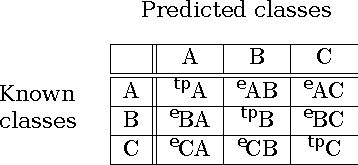
\includegraphics[width=0.3\textwidth]{images/methodology/confusionMatrixCalc.pdf}
    \caption{A simple confusion matrix}
    \label{fig:confisionMatixCalc}
\end{figure}

While recall and precision rates can be individually used to determine the quality of a classifier, it is often more convenient to have a single measure to do the same assessment. The F\textsubscript{1} measure combines the recall and precision rates in a single equation:

\[ F\textsubscript{1} = 2\frac{precision*recall}{precision+recall} \]

Because the labelled data was consisting of 1500 traffic tweets and 14505 non-traffic tweets two different training and evaluation have been integrated. 

Firstly, the classifier was trained with 1000 traffic and 1000 non-traffic tweets. Then it was tested with 500 traffic and 500 non-traffic tweets. The metrics for this training are the following. 

Accuracy of the classifier:   0.87

Traffic precision:            0.842592592593
Traffic recall:               0.91
Traffic F-measure:            0.875

Non-Traffic precision:        0.902173913043
Non-Traffic recall:           0.83
Non-Traffic F-measure:        0.864583333333

\begin{figure}[h]
\begin{center}
    \begin{tabular}{| l || c | c | }
    \hline
          & Non-Traffic & Traffic \\ \hline \hline
         Non-Traffic & 41.5\% & 8.5\% \\ \hline
         Traffic & 4.5\% & 45.5\% \\ \hline
    \end{tabular}
    \caption{Confusion Matrix with 1000 traffic and 1000 non-traffic tweets.}
    \label{fig:confusionMatrix1}
\end{center}
\end{figure}	

Secondly, the classifier was trained with 1000 traffic and 9670 non-traffic tweets. Then it was tested with 500 traffic and 4835 non-traffic tweets. The metrics for this training are the following. 

Accuracy of the classifier:   0.862605435801

Traffic precision:            0.401019541206
Traffic recall:               0.944
Traffic F-measure:            0.562909958259

Non-Traffic precision:        0.993265993266
Non-Traffic recall:           0.854188210962
Non-Traffic F-measure:        0.918492160569

\begin{figure}[h]
\begin{center}
    \begin{tabular}{| l || c | c | }
    \hline
          & Non-Traffic & Traffic \\ \hline \hline
        Non-Traffic & 77.4\% & 13.2\% \\ \hline
        Traffic & 0.5\% & 8.8\% \\ \hline
    \end{tabular}
    \caption{Confusion Matrix with 1000 traffic and 9670 non-traffic tweets.}
    \label{fig:confusionMatrix1}
\end{center}
\end{figure}
	
As it can been observed from the confusion matrices, with the first training it has been achieved a rather bad accuracy since 19\% of the non-traffic tweets are being classified wrong and 9\% of the traffic tweets are being classified wrong. On the other hand, with the second training the traffic tweets error has been almost halved to 5\% resulting a more accurate classification for the traffic tweets even if the global accuracy dropped by 1\%. That means the classifier may classified some traffic tweets as non-traffic but it classified much less non-traffic tweets as traffic.

\subsubsection{Functional/Integration Testing}
One of the most important parts of the project was the server API interface. A lot of requests will 
be coming from the mobile application and it must be confirmed that the server interface can handle 
them but also return the expected results using the expected format. In order to test the server 
interface the Apache JMeter desktop application was used. This software is designed to load test 
functional behaviour and measure the performance of static and dynamic recourses. Using JMeter 
proved to be a very effective way to test the servers interface. Various test plans where created 
testing every GET or POST request available to use through the API. These plans where created for 
both the server and the mock server that are running on ports 55004 and 55003 accordingly. More 
tests were implemented to ensure that the server was returning the correct messages and response 
codes when it was encountering an error. In addition, invalid requests to the server had also been 
checked for error handling and if the error messages were displayed correctly into the screen. For 
each request, the content-type was also checked if it evaluates as JSON. This process was really 
helpful because it was very easy later on to check whether new features implemented or code 
refactoring were actually breaking the API. All the test plan configuration settings have been saved 
in the project repository as a .jmx file. 

\subsubsection{Unit Testing} 

